\section{Cartograms with Dynamic Features}

{
\begin{figure}[tb!]
    \centering
    \includegraphics[width=\columnwidth]{example-image-a}
    \caption{An screenshot of \software. Figure TBA.}
    \label{fig:overview}
\end{figure}
}

{
    \begin{figure}[tb!]
        \centering
        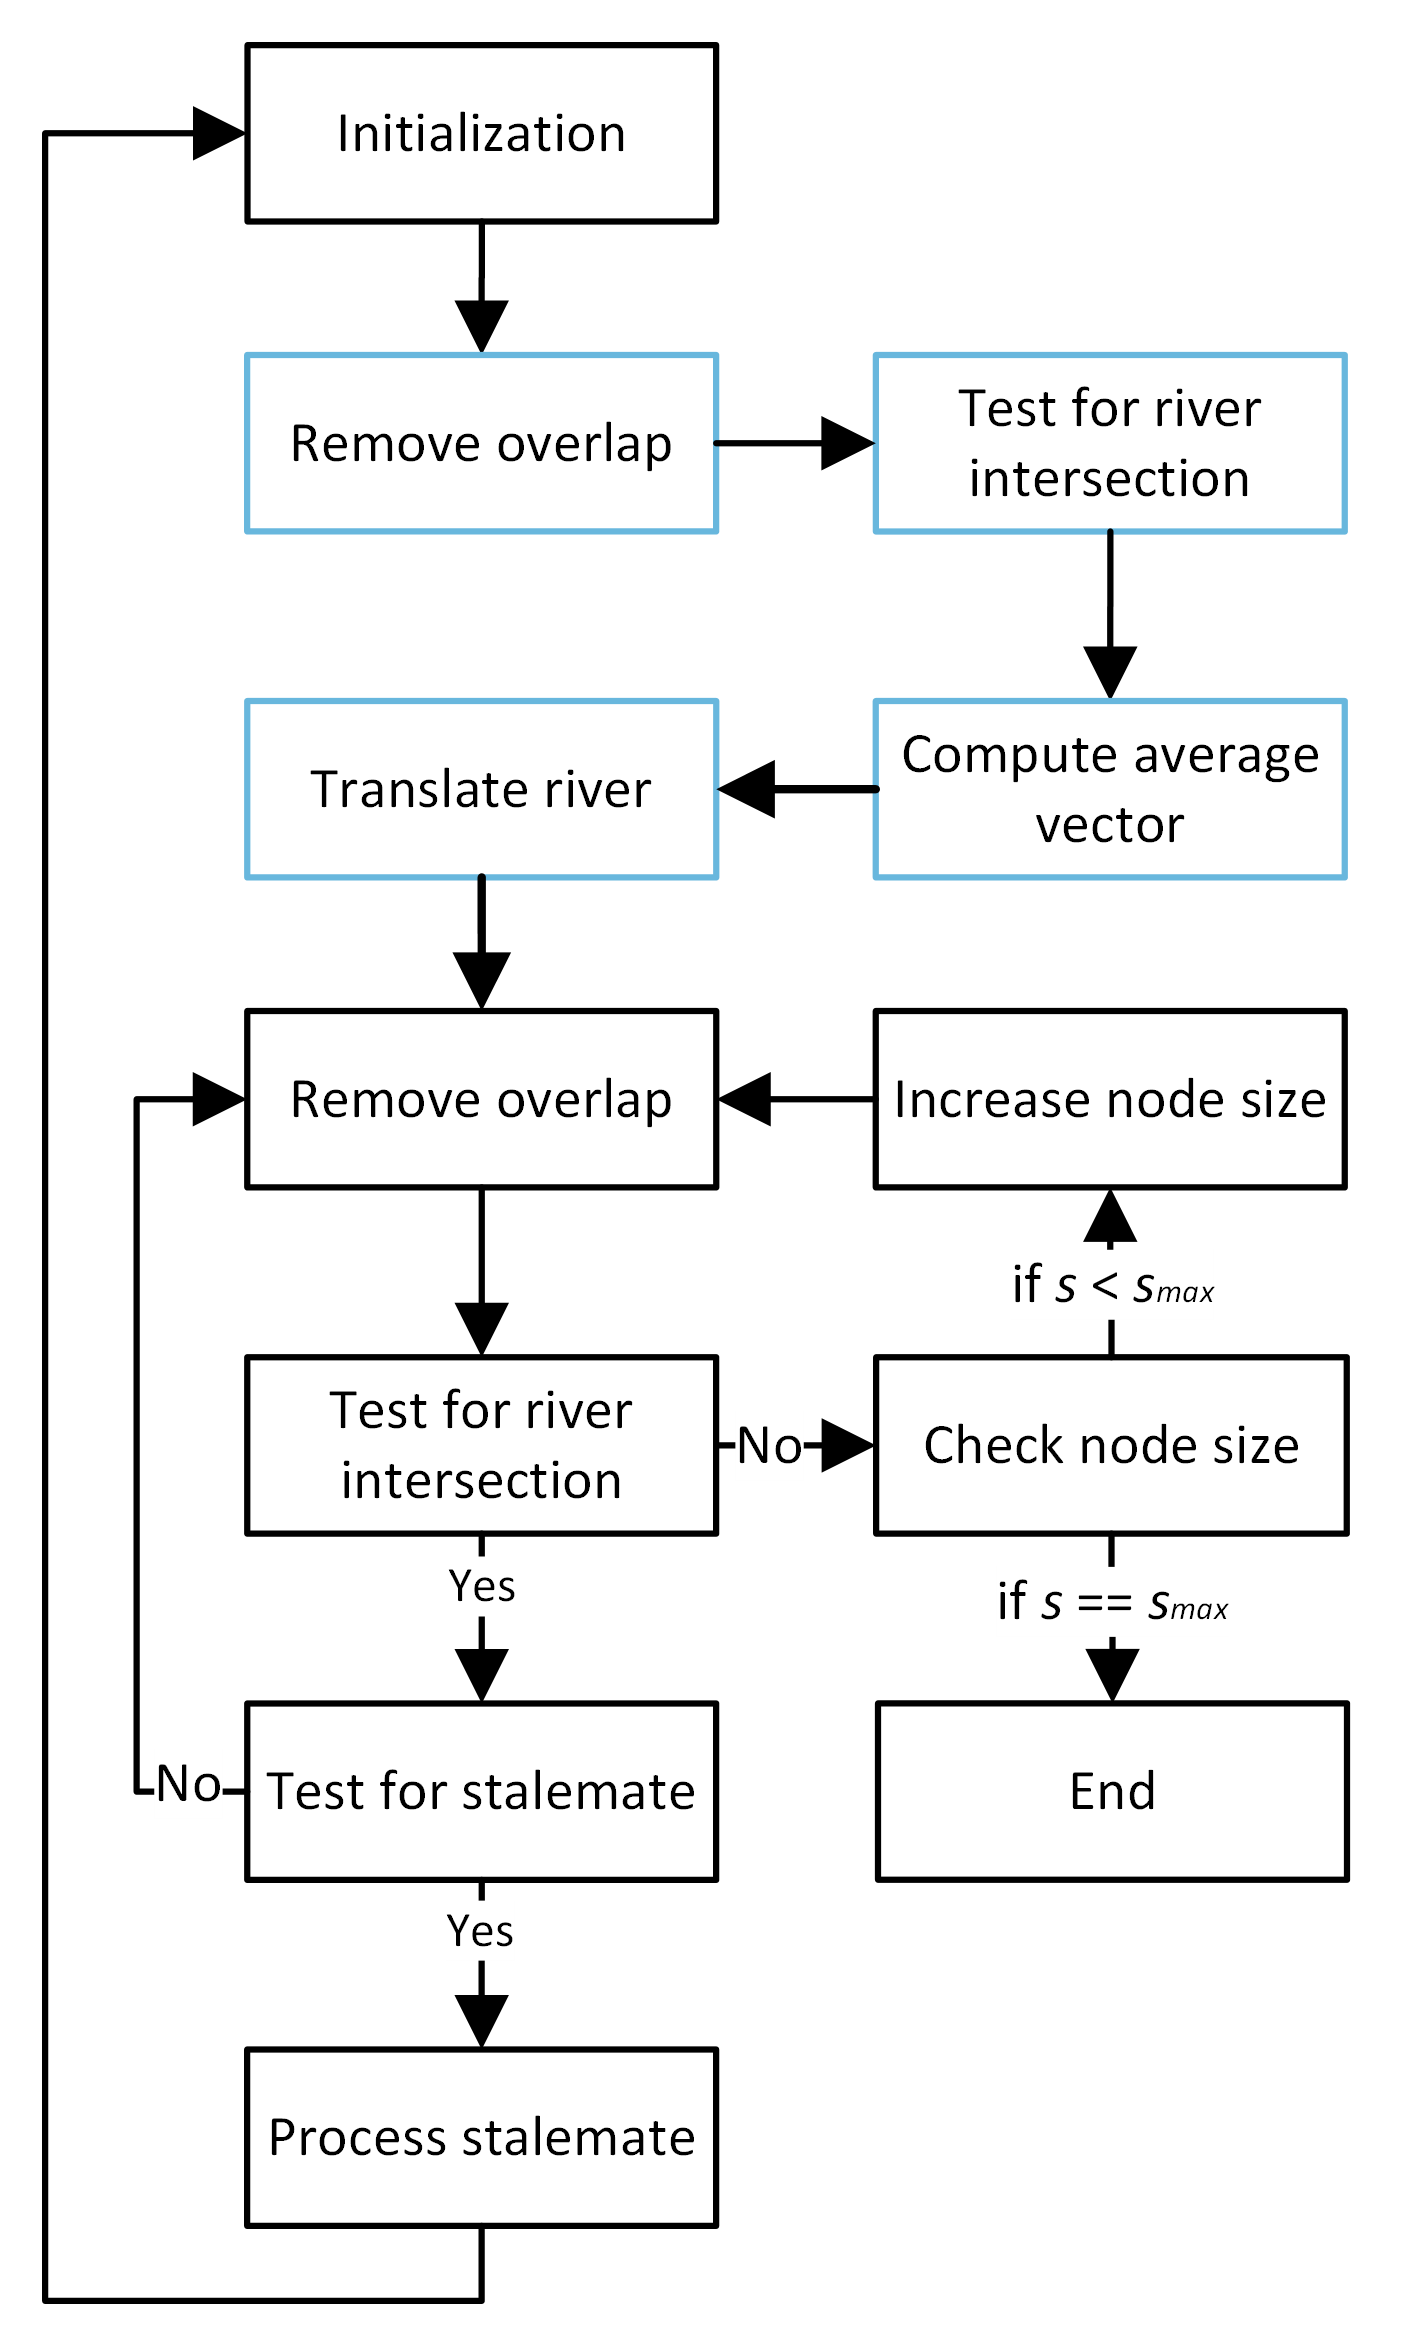
\includegraphics[width=0.8\columnwidth]{figure/flowchart.png}
        \caption{A flowchart illustration of our layout algorithm.See \figref{fig:flowchart-stalemate} for the flow of processing stalemate. See also \algoref{alg:UpdateNodePosition} for more detail.}
        \label{fig:flowchart}
    \end{figure}

    \begin{figure}[tb!]
        \centering
        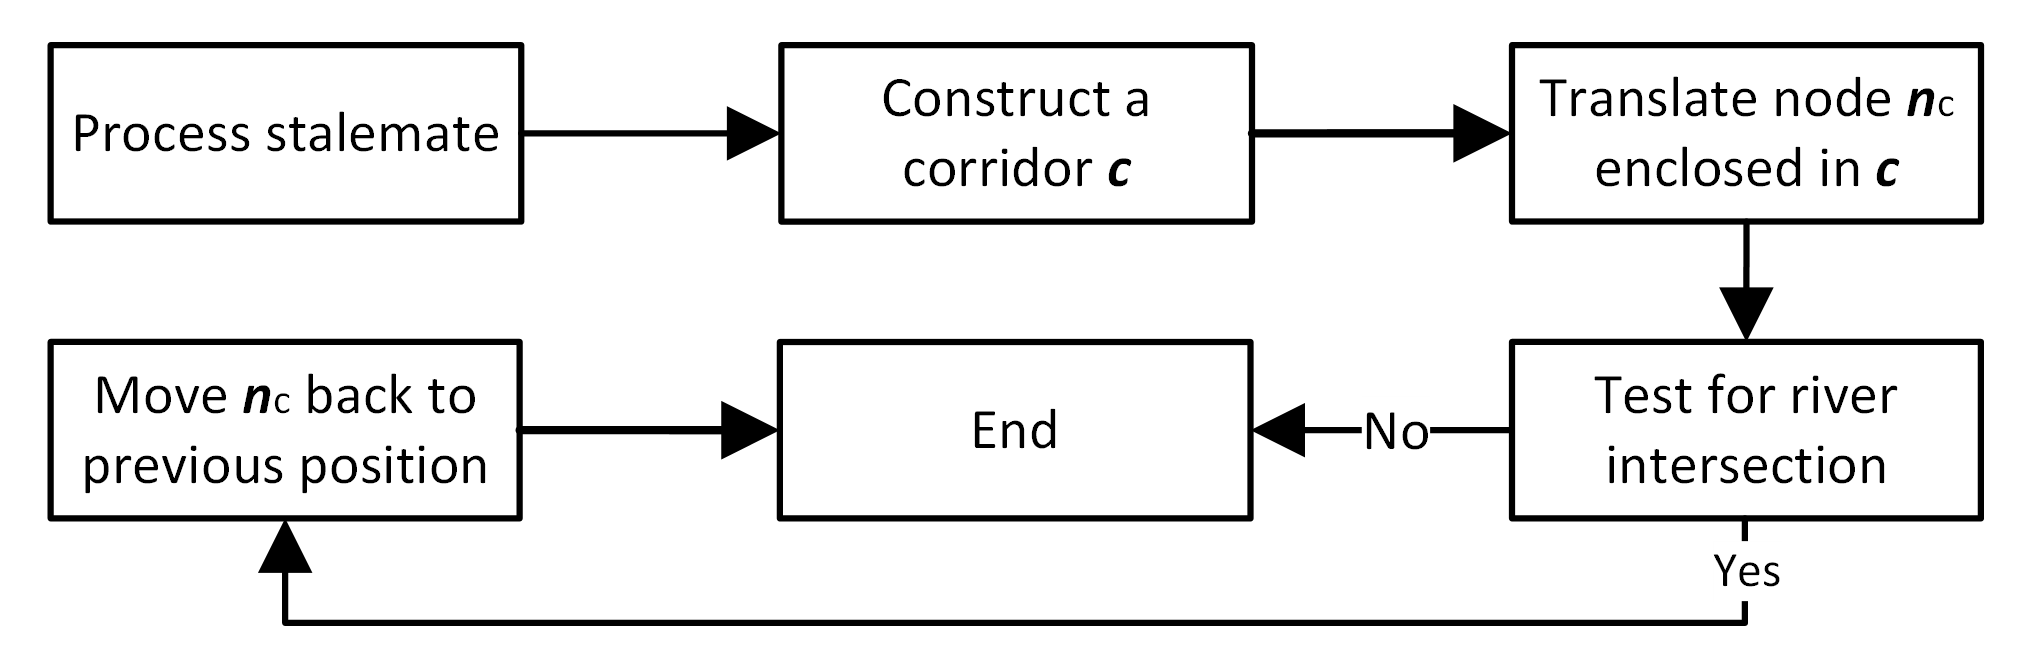
\includegraphics[width=0.9\columnwidth]{figure/flowchart stalemate.png}
        \caption{A flowchart illustration of stalemate processing.}
        \label{fig:flowchart-stalemate}
    \end{figure}
}

\algoref{alg:UpdateNodePosition} and \figref{fig:flowchart} provide an overview of the process.

\bobgraph{Initialization:} We first load and render the CCG geospatial boundaries. For each CCG we compute the centroid and represent it using a square node, $ \node $, with the initial size, $ \nodeSize $. We then load the river shapefiles and render the rivers. Since the vertices of the river in the shapefiles are not in sequential order, we first render the starting vertex, followed by the next closest vertex. This rendering approach enables us to adjust the river resolution as shown in \figref{fig:river resolution}. We further apply a smoothing logic by removing vertices that are too close to each other.

\bobgraph{Node layout:} The basic algorithm is as follows: we first apply the Fast Node Overlap Removal (FNOR) algorithm that solves the Variable Placement with Separation Constraints (VPSC) problem \cite{dwyer2006fast} in order to remove overlaps. We chose FNOR over other node overlap removal algorithms because FNOR is able to provide spread minimization and node movement minimization while maintaining a good level of global shape preservation \cite{chen2020Node}. We gradually increase the node size by 1 unit at a time to ensure smooth transitions. An increase in $ \nodeSize $ can cause the nodes to overlap. During overlap removal, we compute node trajectories (See \algoref{alg:check river intersection}) and translate nodes to their new position. Nodes that cross a river are translated back to their previous position. If a node oscillates across a river, we process this as a stalemate. This procedure ends when 1) no node overlap is present; 2) no nodes cross a river. We then increase $ \nodeSize $ by one pixel and repeat the algorithm until the max node size $ \nodeSizeMax $ is reached. The gradual size increase process provides stability to the layout and helps minimize geographical error.

% \begin{noindent}

\begin{algorithm}[tb!]
    \caption{Procedure to update node positions by removing overlap and prevent nodes from crossing rivers.}\label{alg:UpdateNodePosition}
    \textbf{Global variables:} \\
    $ \nodeList \gets $ a list of $ \node $ representing CCGs with the following properties: \\
    \-\hspace{1em} $ \nodeListCross \gets True $ if any $ \node $ in $ \nodeList $ crosses a river \\
    $ \nodeSize \gets $ the current size of all nodes \\
    $ \nodeSizeMax \gets $ the maximum size of a node \\
    $ \stalemateMax \gets $ the maximum number of iterations indicating a stalemate \\

    \textbf{Local variables:} \\
    $ \node \gets $ a node is an object with the following properties: \\
    \-\hspace{1em} $ \node.x, \node.y, $ or $ \node(x,y) \gets $ the x and y coordinates of $ \node $ \\
    \-\hspace{1em} $ \nodeCross \gets $ the counter for river crosses for $ \node $ \\
    \-\hspace{1em} $ \nodePrevious \gets $ the previous position of $ \node $ \\
    \-\hspace{1em} $ \nodeFNOR \gets $ the translated position of $ \node $ \\


    \begin{algorithmic}[1]
        \Procedure{UpdateNodePosition}{}
        \While{$ \nodeSize < \nodeSizeMax $}
            \State $ \nodeListCross \gets True $
            \While{$ \nodeListCross = True $}

                \State $ \nodeListCross \gets False $
                \State $ \nodeList \gets $ RemoveOverlap ($ \nodeList $)

                \ForEach {$ \node \in \nodeList $}

                    \If {$ \node(x,y) \neq \nodeFNOR(x,y) $}
                        
                        \State $ \node(x,y) \gets \nodeFNOR(x,y) $

                        \If{ \Call{TestIntersection}{$ \nodeFNORLine $} $ = True $}
                            \State $ \nodeCross \gets \nodeCross ++ $
                            \State $ \nodeListCross \gets True $

                            \If{$ \nodeCross < \stalemateMax $}
                                \State \hskip-2em \Comment{Translate back to previous position}
                                \State $ \node(x,y) \gets \nodePrevious(x,y) $

                            \Else

                                \State \Call{ProcessStalemate}{$ \node, \nodeFNOR $}
                                \State $ \nodeCross \gets 0 $ \Comment{Reset counter}

                            \EndIf
                            
                        \EndIf

                    \EndIf

                \EndFor

            \EndWhile

            \State $ \nodeSize \gets \nodeSize ++$

        \EndWhile

        \EndProcedure
    \end{algorithmic}
\end{algorithm}


%\end{noindent}

% \begin{noindent}

    \begin{algorithm}[tb!]
        \caption{Procedure to adjust river positions, remove node overlap and prevent nodes from crossing rivers.}\label{alg:UpdateLayout}
        \textbf{Global variables:} \\
        $ \nodeList \gets $ a list of $ \node $ representing CCGs with the following properties: \\
        \-\hspace{1em}  \textcolor{blue}{$\nodeListCross \gets $ the number of $ \node $ in $ \nodeList $ that crosses a river} \\
        $ \nodeSize \gets $ the current size of all nodes \\
        $ \nodeSizeMax \gets $ the maximum size of a node \\
        \textcolor{blue}{ $ \riverList \gets $ a list of $ \river $ representing river features} \\
        $ \stalemateMax \gets $ the maximum number of iterations indicating a stalemate \\

        \textbf{Local variables:} \\
        $ \node \gets $ a node is an object with the following properties: \\
        \-\hspace{1em} $ \node.x, \node.y, $ or $ \node(x,y) \gets $ the x and y coordinates of $ \node $ \\
        \-\hspace{1em} $ \nodeCross \gets $ the counter for river crosses for $ \node $ \\
        \-\hspace{1em} $ \nodePrevious \gets $ the previous position of $ \node $ \\
        \-\hspace{1em} $ \nodeFNOR \gets $ the translated position of $ \node $ \\

        \begin{algorithmic}[1]
            \Procedure{UpdateLayout}{}
            \While{$ \nodeSize < \nodeSizeMax $}
                \State \textcolor{blue}{$ \nodeListCross \gets 1 $ \Comment{Trigger the while loop}}
                \While{$ \nodeListCross > 0 $}

                    \State $ \nodeListCross \gets 0 $
                    \State $ \nodeList \gets $ RemoveOverlap ($ \nodeList $)
                    \color{blue}
                    \ForEach {$ \river \in \riverList $}
                        \State $ \riverVector \gets (0,0) $ \Comment{Hold the sum of vectors $ \nodeVectorCT $}
                        \ForEach {$ \node \in \nodeList $}

                            \If {$ \node(x,y) \neq \nodeFNOR(x,y) $}
                                \If{ \Call{TestIntersection}{$ \nodeFNORLine $, $ \river $} $ = True $}
                                \State $ \riverVector \gets \riverVector + \nodeVectorCT$
                                \State $ \nodeListCross \gets \nodeListCross ++ $
                                \EndIf

                            \EndIf

                        \EndFor

                        \State Translate river $ \river $ by the average vector $ \frac{\riverVector}{\nodeListCross} $
                        \State $ \nodeListCross \gets 0 $ \Comment{Clear the counter}
                    \EndFor


                    \color{black}
                    \ForEach {$ \node \in \nodeList $}
    
                        \If {$ \node(x,y) \neq \nodeFNOR(x,y) $}
                            
                            \State $ \node(x,y) \gets \nodeFNOR(x,y) $
    
                            \If{ \Call{TestIntersection}{$ \nodeFNORLine $} $ = True $}
                                \State $ \nodeCross \gets \nodeCross ++ $
                                \State $ \nodeListCross \gets \nodeListCross++ $
    
                                \If{$ \nodeCross < \stalemateMax $}
                                    \State \hskip-2em \Comment{Translate back to previous position}
                                    \State $ \node(x,y) \gets \nodePrevious(x,y) $
    
                                \Else
    
                                    \State \Call{ProcessStalemate}{$ \node, \nodeFNOR $}
                                    \State $ \nodeCross \gets 0 $ \Comment{Reset counter}
    
                                \EndIf
                                
                            \EndIf
    
                        \EndIf
    
                    \EndFor
    
                \EndWhile
    
                \State $ \nodeSize \gets \nodeSize ++$
    
            \EndWhile
    
            \EndProcedure
        \end{algorithmic}
    \end{algorithm}
    
    
%\end{noindent}

\subsection{River Intersection Testing}

We use rivers as topological boundaries and prevent nodes from crossing them. The resolution of rivers can be adjusted by the user, as shown in \figref{fig:river resolution}, the number of vertices is reduced from 10,170 to 30. A pixel-level river resolution is not required as Demers cartograms do not need to represent geography at this level of detail. Instead a resolution that matches the node size is used. Enabling river simplification reduces the number of edge intersection tests that need to be performed. When a node's position changes, we test if the node's trajectory intersects any segment of a river. See \algoref{alg:check river intersection}. A bounding box intersection test between the edge defined by node translation and river edges can be performed to reduce the number of edge intersection tests required.


{
\begin{figure}[tb!]
    \centering
    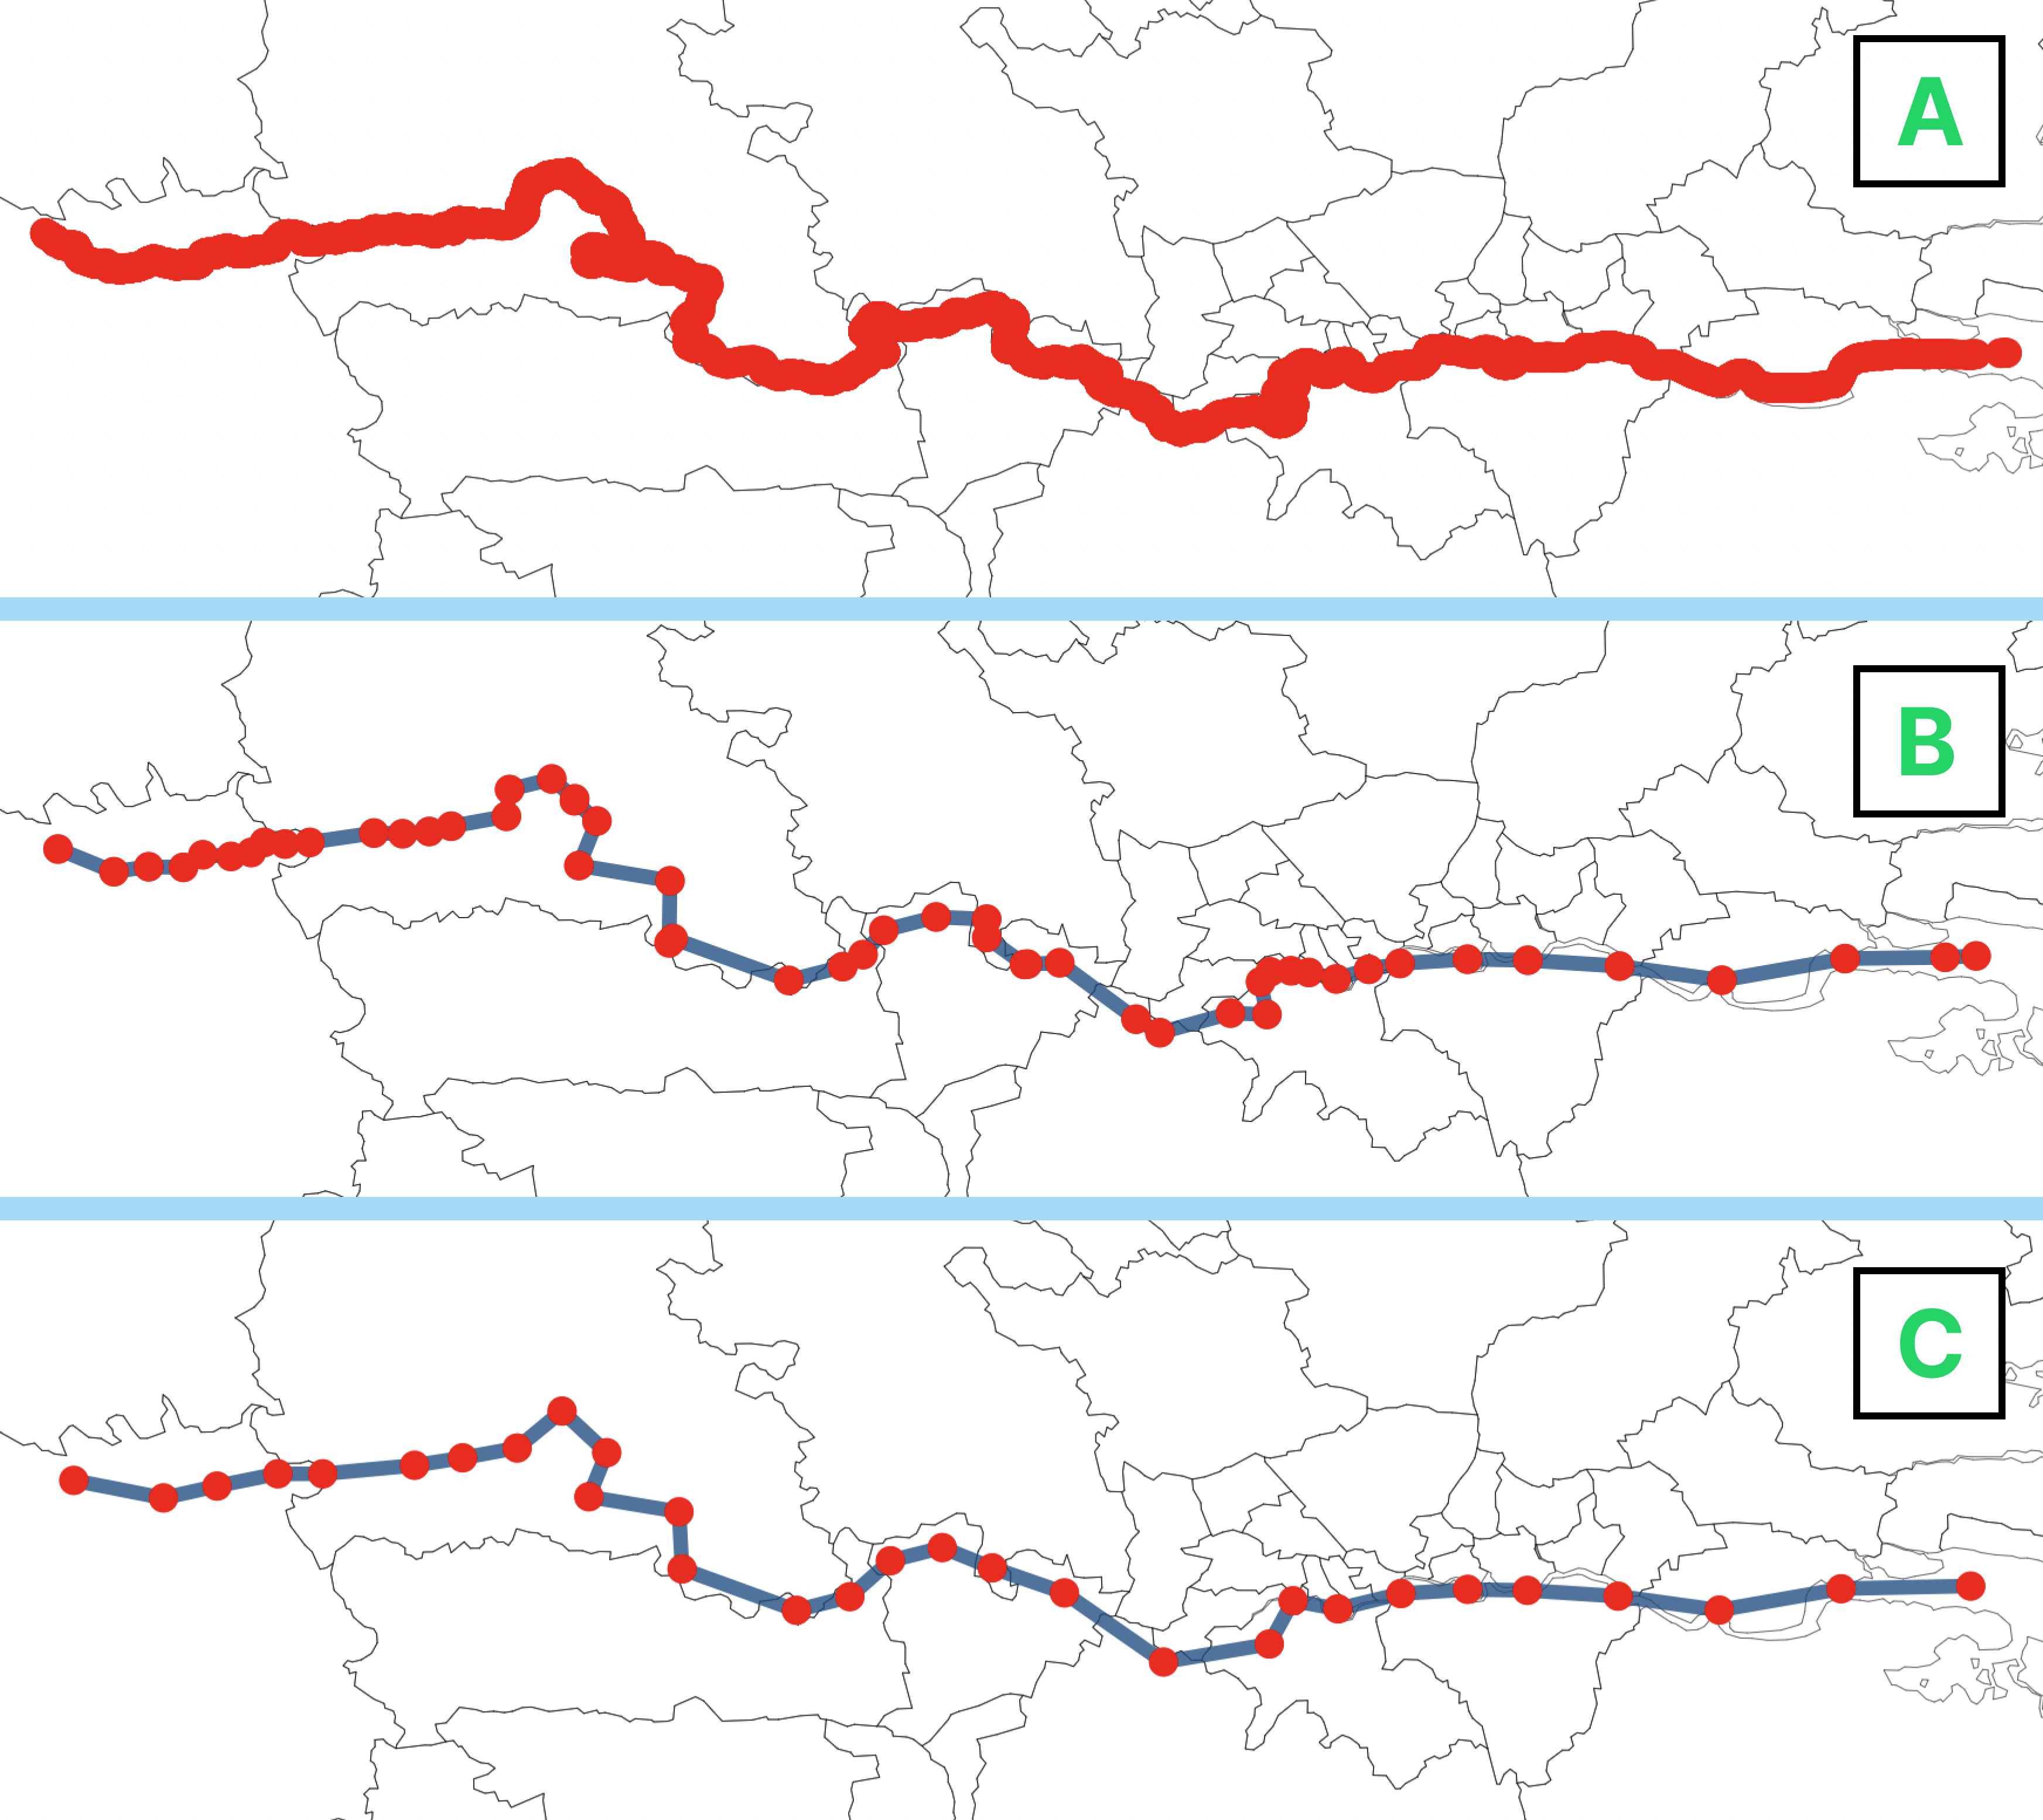
\includegraphics[width=\columnwidth]{figure/river_resolution.png}
    \caption{The resolution of rivers can be dynamically adjusted by the user. A shows River Thames at its original resolution with 10,170 edges. B shows the river at a reduced resolution of 49 edges. We further smooth the river by removing vertices in dense areas, as shown in C. The reduced resolution preserves the majority of River Thames' original shape and improves the performance of our river intersection tests.}
    \label{fig:river resolution}
\end{figure}
}

% \begin{noindent}
\begin{algorithm}[tb!]
    \caption{Procedure to test if a node's translation path, $ \nodeLineNV $ intersects a river.}\label{alg:check river intersection}
    \textbf{Input:} \\
    $ \nodeLineNV \gets $ the node's translation path \\
    $ \river \gets $ a river feature \\

    \textbf{Output:} \\
    Returns $ True $ if the node crosses a river. \\

    \textbf{Local variables:} \\
    $ \nodeBoundingBox, \riverEdgeBoundingBox \gets $ the bounding boxes for $ \nodeLineNV $ and $ \Edge $ \\
    $ \Edge \gets $ an edge of $ \river $ \\

    \begin{algorithmic}[1]
        \Procedure{TestIntersection}{$ \nodeLineNV $, $ \river $}
        
        \ForEach{$ \Edge \in \river $}
            \State $ \nodeBoundingBox \gets $ GetBoundingBox ($ \nodeLineNV $)
            \State $ \riverEdgeBoundingBox \gets $ GetBoundingBox ($ \Edge $)

            \If{$ \nodeBoundingBox ~intersect~ \riverEdgeBoundingBox = True $}
                \State \Return{$ \nodeLineNV ~intersect~ \Edge $}
                \EndIf
        \EndFor
        
        \State \Return{$ False $}
        \EndProcedure
    \end{algorithmic}
\end{algorithm}
%\end{noindent}

\subsection{Detecting Stalemates}

As the FNOR always attempts to produce an optimal node layout where node distribution and translation are minimized, a node's translation path can repeatedly intersect a river due to congestion, creating a stalemate situation, as shown in \figref{fig:stalemate}. If a node is translated between two positions, $ \node $ and $ \nodeFNOR $, for $ \stalemateMax $ iterations (a user-adjustable parameter), we introduce a heuristic solution: constructing a corridor to alleviate the congestion. A corridor, $ \Corridor $, is a rectangle with a width of $ \CorridorWidth $ and a length of $ \CorridorLength $, formed by deriving two edges $ \EdgeParallelA $ and $ \EdgeParallelB $ such that $ \EdgeParallelA \parallel \EdgeParallelA \parallel \nodeLineNtNc $ (See \figref{fig:corridor}C and D). All nodes enclosed by $ \Corridor $ are then translated by $ \nodeVectorTC $ to alleviate the congestion (See \figref{fig:corridor}E).

{
\begin{figure}[tb!]
    \centering
    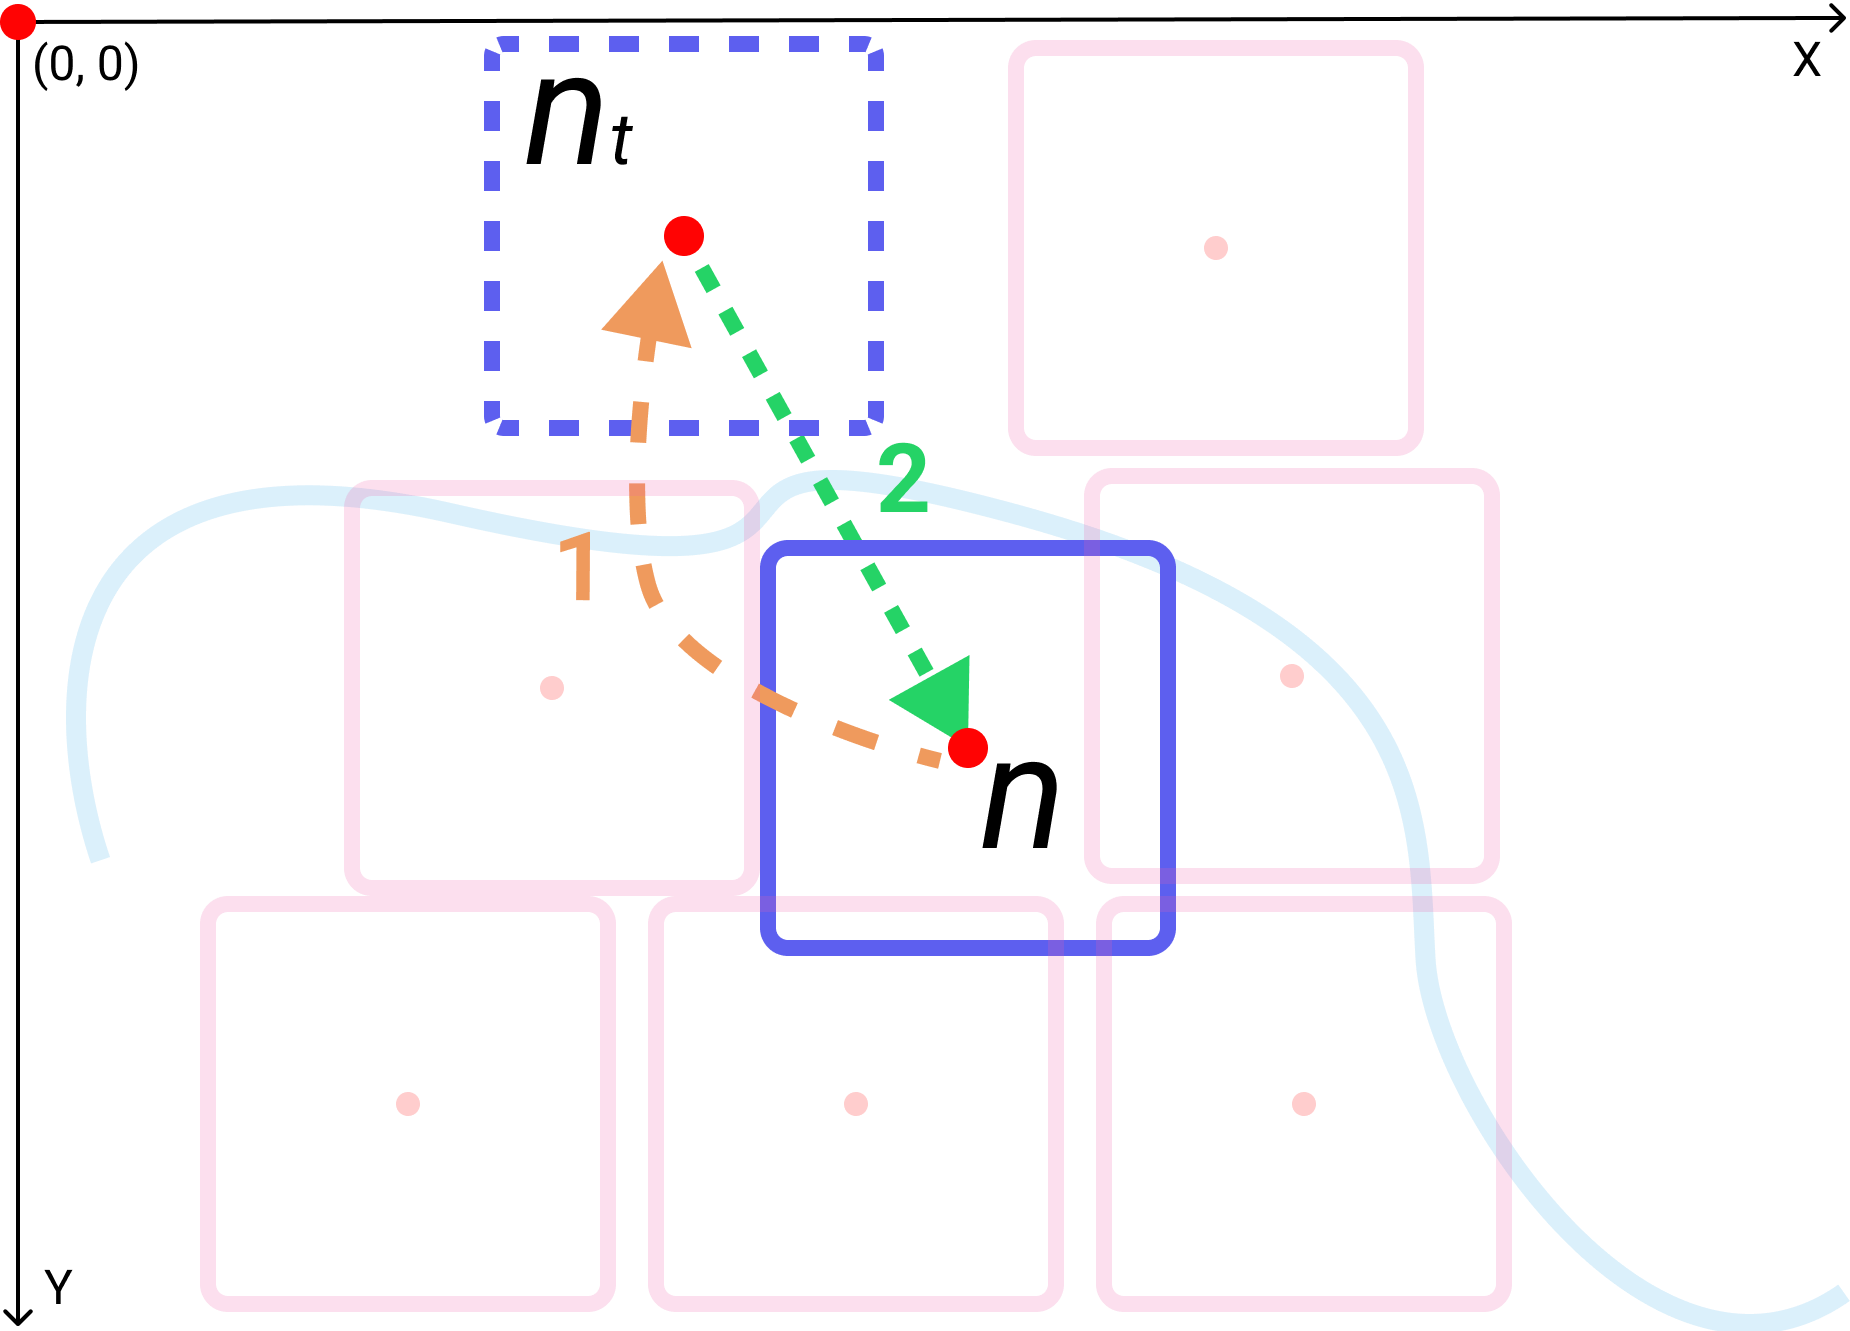
\includegraphics[width=\columnwidth]{figure/stalemate.png}
    \caption{A stalemate situation is when a node's translation path $ \nodeVectorCT $ (in iteration 1) intersects a river $ \stalemateMax $ times. The node is translated back to its previous position (iteration 2). A stalemate often occurs when the area is congested and the node is unable to translate to a new position without intersecting a river.}
    \label{fig:stalemate}
\end{figure}
}

{
\begin{figure}[tb!]
    \centering
    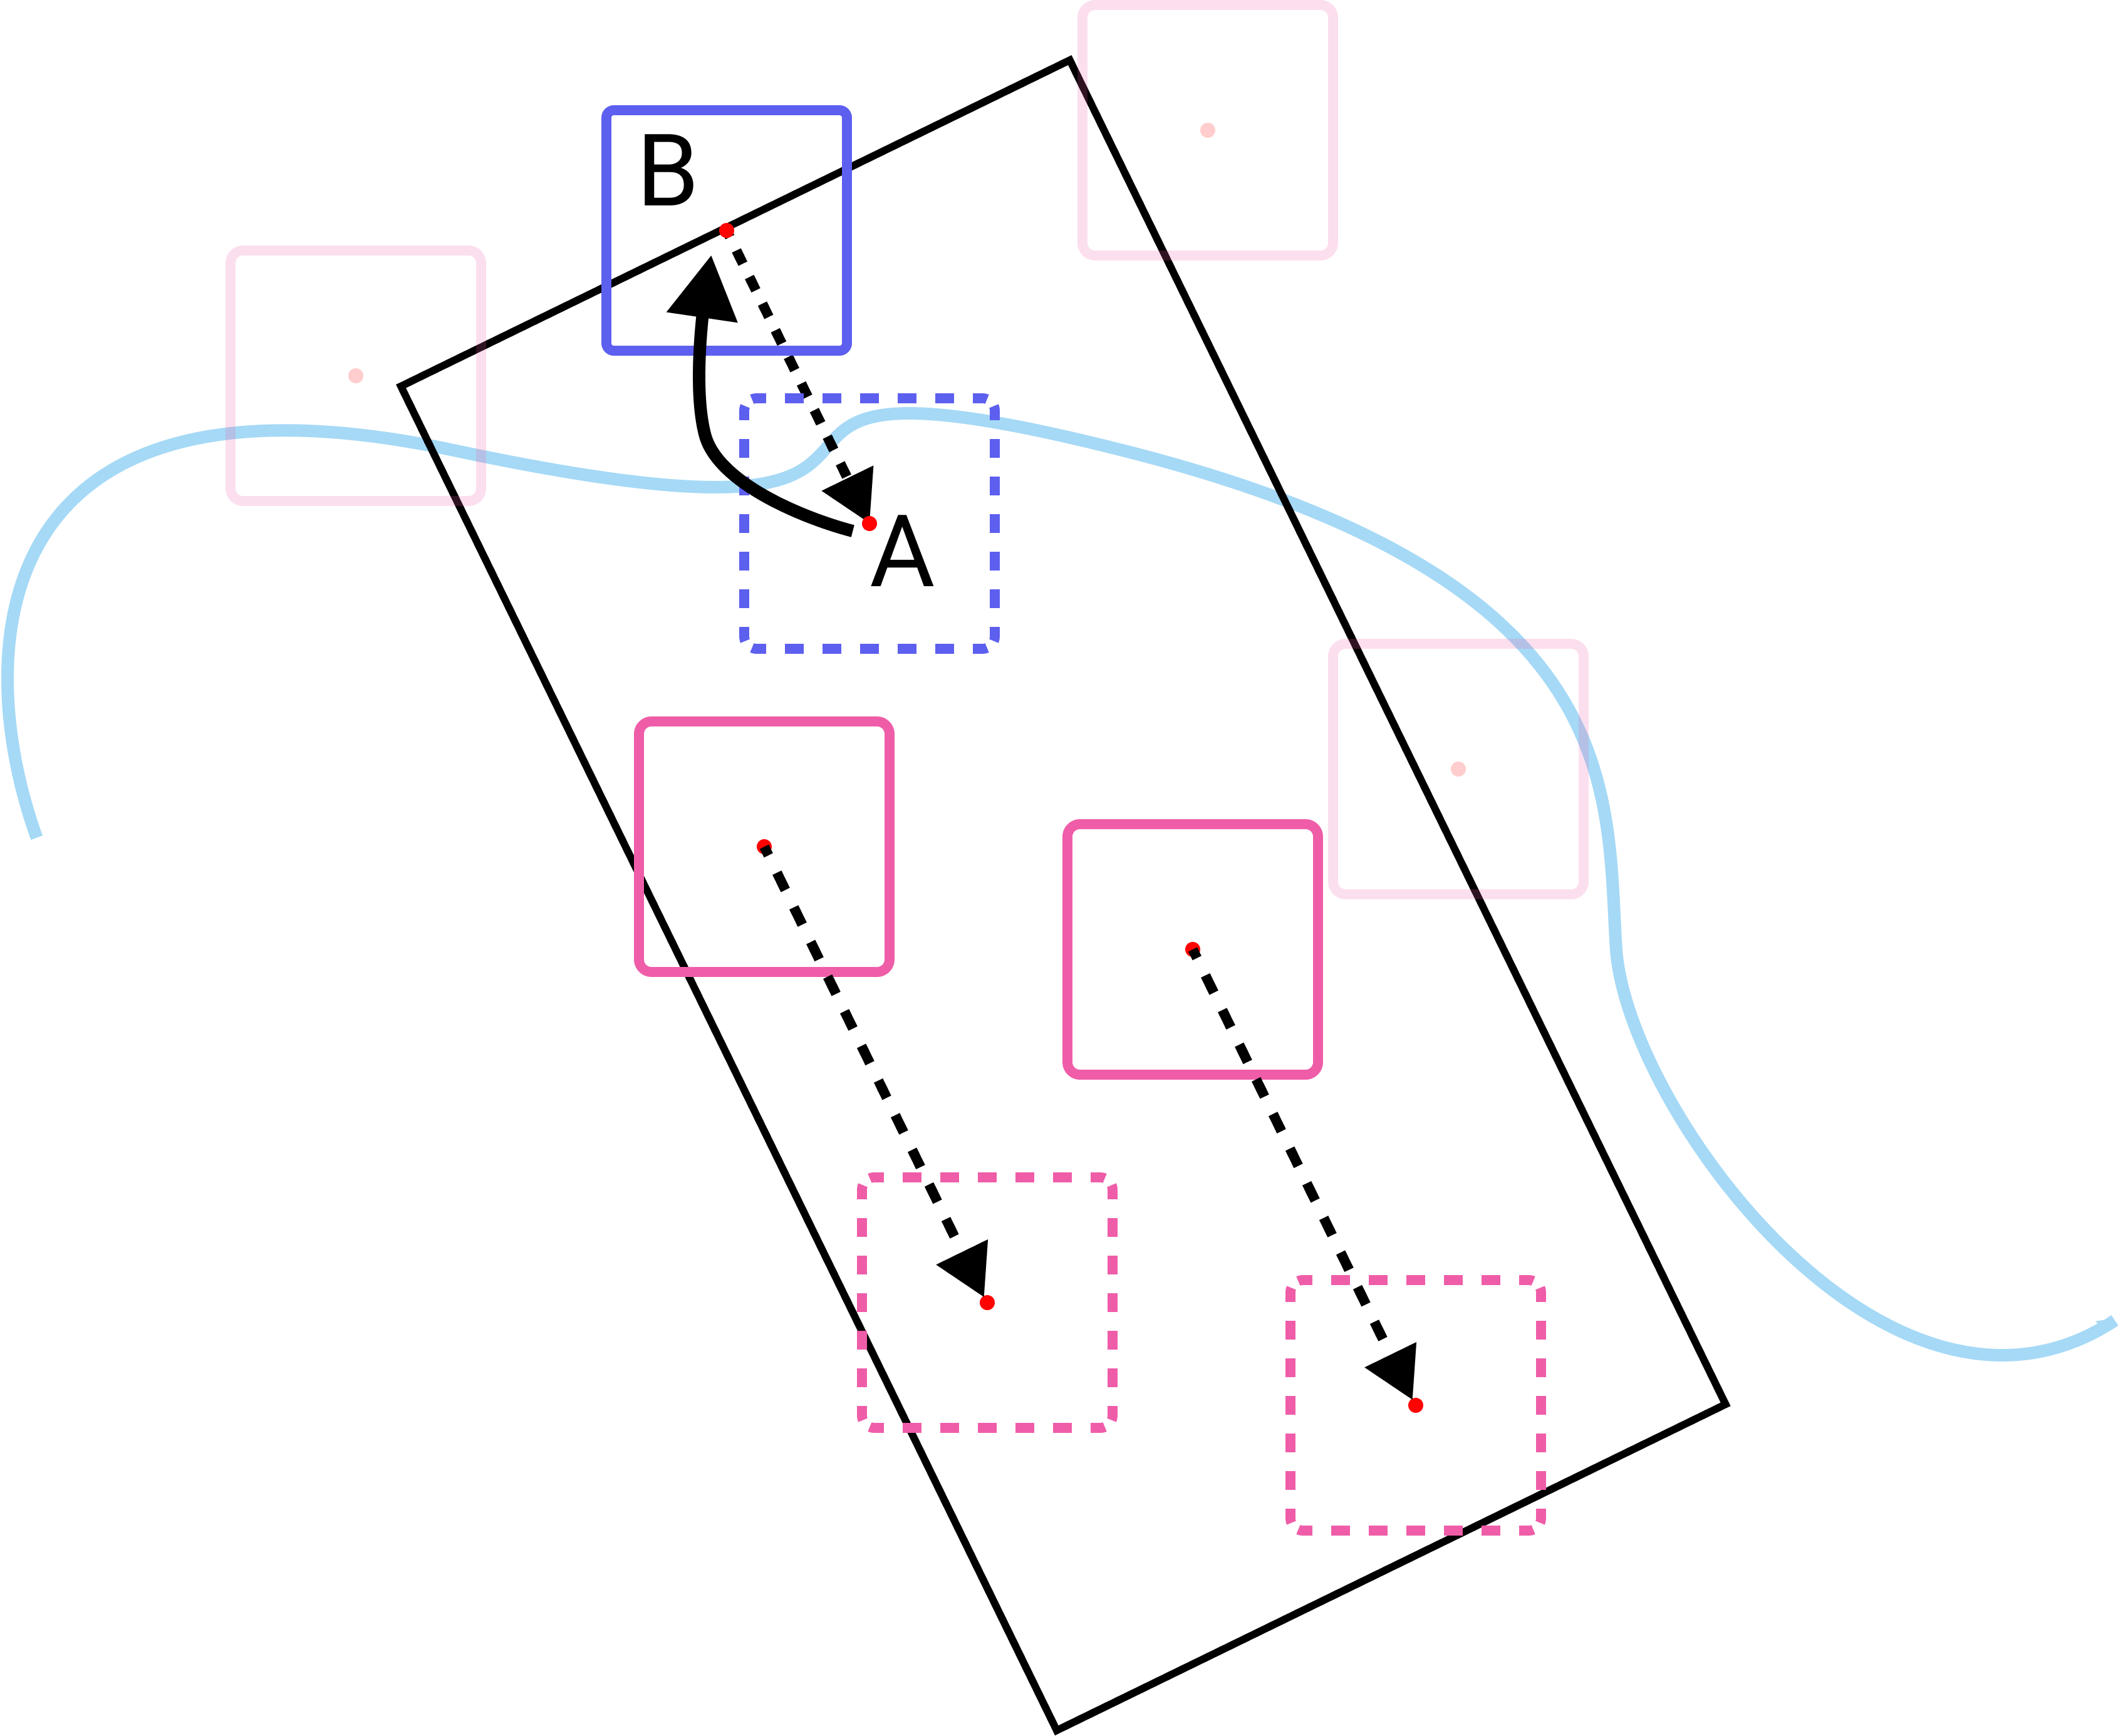
\includegraphics[width=\columnwidth]{figure/corridor.png}
    \caption{A stalemate occurs when a node's translation path $ \nodeVectorCT $ intersects a river for $ \stalemateMax $ times, as shown in A. To address the issue, we derive a corridor (orange rectangle in E) based on $ \node $ and $ \nodeFNOR $. All nodes within the corridor are translated based on $ \nodeVectorTC $, such that $ \nodeVectorNNn = \nodeVectorNinNinn $. In order to show a clear illustration, we place nodes sparsely in this figure.}
    \label{fig:corridor}
\end{figure}
}

% \begin{noindent}

\begin{algorithm}[tb!]
    \caption{Procedure to derive a corridor to translate enclosed nodes. We use an SVG canvas, where the point of origin (0,0) is located at the top left corner, with the x-axis extending to the right and the y-axis extending downwards (See \figref{fig:stalemate}).}\label{alg:derive corridor}

    \textbf{Input:} \\
    $ \node \gets $ the node used to derive the corridor \\

    \textbf{Global variables:} \\
    $ \CorridorLength \gets $ the length of a corridor \\
    $ \CorridorWidth \gets $ the width of a corridor \\

    \textbf{Local variables:} \\
    $ \Corridor \gets $ the corridor \\
    $ \PointP \gets $ the point extending $ \nodeVectorTC $ such that $ \nodeLineWidthNtP = \CorridorLength $\\
    $ \EdgeParallelA, \EdgeParallelB \gets $ the edges parallel to $ \nodeLineNtNc $ \\
    $ corridor \gets $ a rectangle formed by $ \EdgeParallelA $ and $ \EdgeParallelB $ \\

    \begin{algorithmic}[1]
        \Procedure{ProcessStalemate}{$ \node $}
            \State $ \node(x,y) \gets \nodePrevious(x,y) $

            \State $ \PointP \gets $ \Call{DerivePoint}{$ \nodeVectorTC $, $ \CorridorLength $}

            \State $ \EdgeParallelA \gets $ \Call{DeriveParallelEdge}{$ \nodeVectorNtP $, $ \frac{\CorridorWidth}{2} $}

            \State $ \EdgeParallelB \gets $ \Call{DeriveParallelEdge}{$ \nodeVectorNtP $, $ -\frac{\CorridorWidth}{2} $}

            \State $ \Corridor \gets
                \begin{bmatrix}
                    \EdgeParallelA.start &
                    \EdgeParallelA.end \\

                    \EdgeParallelB.start &
                    \EdgeParallelB.end \\
                \end{bmatrix} $

            \ForEach{$ \nodeInCorridor $ inside $ \Corridor $}

                \State $ \Vector{\nodeInCorridor ~\nodeInCorridorT} = \nodeVectorTC $

                \State $ \nodeInCorridor(x,y) \gets \nodeInCorridorT(x,y) $

            \EndFor
        \EndProcedure
    \end{algorithmic}
\end{algorithm}

%\end{noindent}
